\documentclass{article}
\usepackage[margin=1in]{geometry}
\usepackage{amsmath,amsthm,amssymb}
\usepackage{bbm,enumerate,mathtools}
\usepackage{tikz,pgfplots}
\usepackage{chessboard}
\usepackage[hidelinks]{hyperref}
\usepackage{multicol} % Problem 35
\usepackage{xstring} % Difficulty command
\usetikzlibrary{shapes.geometric}

\newenvironment{question}{\begin{trivlist}\item[\textbf{Question.}]}{\end{trivlist}}
\newenvironment{note}{\begin{trivlist}\item[\textbf{Note.}]}{\end{trivlist}}
\newenvironment{references}{\begin{trivlist}\item[\textbf{References.}]}{\end{trivlist}}
\newenvironment{related}{\begin{trivlist}\item[\textbf{Related.}]\end{trivlist}\begin{enumerate}}{\end{enumerate}}

\newcommand\score[1]{
\pgfmathsetmacro\pgfxa{#1+1}
\tikzstyle{scorestars}=[
  star,
  star points=5,
  star point ratio=2.25,
  draw,
  inner sep=3pt,
  anchor=outer point 5
]
  \begin{tikzpicture}[baseline]
    \draw[opacity=0] (0,-0.5) rectangle (0,0.2); % Workaround for whitespace at the bottom.
    \foreach \i in {1,...,4} {
      \pgfmathparse{(\i<=#1?"yellow":"gray")}
      \edef\starcolor{\pgfmathresult}
      \draw (\i*4.5ex,0) node[name=star\i,scorestars,fill=\starcolor]  {};
    }
  \end{tikzpicture}
}

\newcommand{\difficulty}[1]{%
  \IfEqCase{#1}{%
      {1}{
        
\begin{tikzpicture}[scale=0.7, baseline=0.9mm]%
          \definecolor{slopegreen}{rgb}{0.0, 0.5, 0.0}%
          \fill[slopegreen] (0.5,0.5) circle (0.5);%
        \end{tikzpicture}%
      }%
      {2}{
        
\begin{tikzpicture}[scale=0.7, baseline=0.9mm]%
          \definecolor{slopeblue}{rgb}{0.0, 0.44, 1.00}
          \fill[slopeblue] (0,0) rectangle (1,1);%
        \end{tikzpicture}%
      }%
      {3}{
\begin{tikzpicture}[scale=0.7, baseline=0.9mm]\fill (0,0.5)--(0.5, 0)--(1,0.5)--(0.5,1)--cycle; \end{tikzpicture}}%
      {4}{
\begin{tikzpicture}[scale=0.7, baseline=0.9mm]\fill (0.25,0)--(0,0.5)--(0.25,1)--(0.5,0.5)--cycle; \fill (0.75,0)--(0.5,0.5)--(0.75,1)--(1,0.5)--cycle;\end{tikzpicture}}%
      % you can add more cases here as desired
  }[\PackageError{difficulty}{Undefined difficulty level: #1}{}]%
}%
\newcommand{\rating}[2]{\difficulty{#1}\\\score{#2}\\}


\begin{document}
\rating{1}{1}
Jeremy Kun gives a canonical bijection between $\displaystyle\binom{n + 1}{2}$ and a discrete
tringle of length $n$, as seen below.
\begin{figure}[!h]
  \centering
  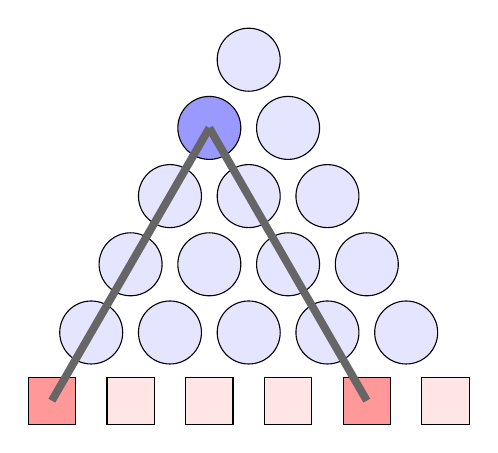
\begin{tikzpicture}
    \foreach \x/\y/\color in {
      0/3/10,
      0/2/40, 1/2/10,
      0/1/10, 1/1/10, 2/1/10,
      0/0/10, 1/0/10, 2/0/10, 3/0/10,
      0/-1/10, 1/-1/10, 2/-1/10, 3/-1/10, 4/-1/10} {
        \draw[fill=blue!\color] ({\x + \y/2}, {sqrt(3)*\y/2}) circle (0.4cm);
      }

      \foreach \x/\y/\color in {
        0/-2/40, 1/-2/10, 2/-2/10, 3/-2/10, 4/-2/40, 5/-2/10} {
          \draw[fill=red!\color]
            ({\x + \y/2 - 0.3}, {sqrt(3)*\y/2 - 0.3})
            rectangle
            ({\x + \y/2 + 0.3}, {sqrt(3)*\y/2 + 0.3});
        }

      \draw[line width=0.1cm, black!60] (1, {sqrt(3)})--(-1, {-sqrt(3)});
      \draw[line width=0.1cm, black!60] (1, {sqrt(3)})--(3, {-sqrt(3)});

  \end{tikzpicture}
  \caption{Bijection that maps a point on the triangle with side length 5 to a 2-subset of [5 + 1].}
\end{figure}

\begin{question}
  Is there a similar ``projection'' that bijects a point on the discrete
  tetrahedron to a \linebreak
  3-subset of [n + 2]?
\end{question}

\begin{note}
  Misha Lavrov gives a potential function to the question on Math Stack Exchange.
\end{note}

\begin{related}
  \item More generally is there a bijection from the $k$-simplex to a $k$-subset of [n + k - 1]?
\end{related}

\begin{references}
  \item \url{https://jeremykun.com/2011/10/02/n-choose-2/}
  \item \url{https://math.stackexchange.com/a/2468687/121988}
\end{references}
\end{document}
